\chapter{Future Work}
\label{ch:future}

\section{Configuration file generation}

The GPRM framework uses YAML configuration files\cite{yaml} when compiling the GPIR code.
An example file for the MergeSort implementation is as follows:

\begin{lstlisting}[language=yaml]

# Core Services Configuration
System:
  Version: 3.0
  Libraries: [MergeSort, CoreServices]
  NServiceNodes: 241 # excluding gateway; this is actually the number of threads
  ServiceNodes:
    ctrl: [ 1, [CoreServices.SEQ ] ]
    control: [ 1, [CoreServices.BEGIN] ]
    a: [ 2, [CoreServices.ALU] ]
    reg: [ 2, [CoreServices.REG ] ]
    MS: [2, [MergeSort.MergeSort] ]

  Aliases:
  # Alias Name (case sensitive): FQN
    begin: control.CoreServices.BEGIN.begin
    par: ctrl.CoreServices.BEGIN.begin
    seq: ctrl.CoreServices.SEQ.seq
    'reg.write': reg.CoreServices.REG.write
    'reg.read': reg.CoreServices.REG.read
    'reg.inc': reg.CoreServices.REG.inc
    'MS.array': MS.MergeSort.MergeSort.array
    'MS.serial_ms': MS.MergeSort.MergeSort.serial_ms
    'MS.merge_two': MS.MergeSort.MergeSort.merge_two
# These used to be "ALU_names"  
    '+': a.CoreServices.ALU.plus
    '*': a.CoreServices.ALU.times
\end{lstlisting}

The YAML file defines what libraries and services are required to be compiled,
number of threads, and aliases for functions in the GPIR code.

It is entirely possible to generate this information from the GPC compiler rather
than manually having to create these files.


\section{Language Features}
    There are many ways the GPC language can be extended to have more
    functionality. A couple of notable features are:
    \begin{itemize}
        \item C++11 lambdas - giving the language the ability to implement higher order functions.
        \item Templates - giving the ability to use some C++ Standard Template Library structures such as Vectors.
        \item Header/Module system - currently a GPC source file has no way of including GPC code
    from other files.

    \end{itemize} 

\section{Compiler Optimisations}

    There are a few optimisations that can be performed by the compiler to reduce the work needed to be 
    performed by the GPRM at runtime.

\subsection{Binary Expression Reduction}
Given the following GPC code:    

\lstinputlisting[style=myGPC]{code_samples/binaryOp.gpc}

The expression within the \texttt{test.m2} method is read in as a binary expression
tree which can be represented by the following:

\begin{center}
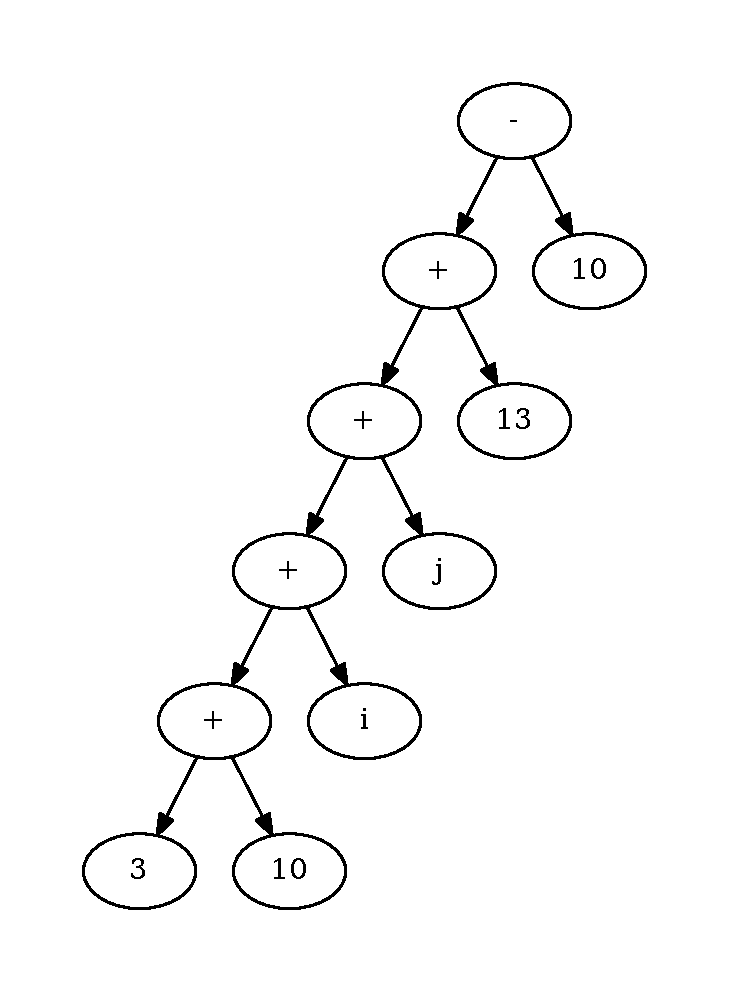
\includegraphics[scale=0.5]{graphs/evalTree.pdf}
\end{center}

The tree above once evaluated transforms into the following tree: 

\begin{center}
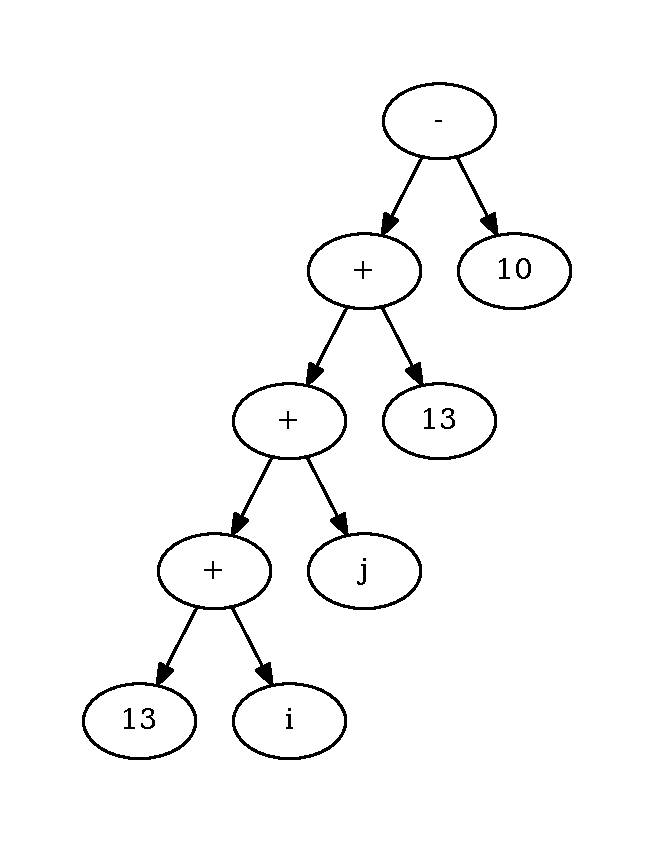
\includegraphics[scale=0.5]{graphs/futureTree.pdf}
\end{center}

We can see this reduction in the generated GPIR code:

\lstinputlisting[style=myGPIR]{code_samples/binaryOp.td}

This shows the limitations of the expression evaluation explained in section ~\ref{sub:partial}.
Once a value that can't be worked out at compile time is met, it is not possible
to evaluate expressions any value further up the tree. In the given example
it is clear that it is possible to evaluate the expression further.

One way to improve the evaluator would be to transform the tree before evaluating it.
Using the axioms of the binary operations in the tree (e.g. addition being associative)
and the type of values in the leaf nodes,. it should be possible to rearrange the nodes in the 
tree to create a new tree which represents an expression equivalent to the expression
represented by the starting tree.

The specific details of how the tree transformations work and implementation into the compiler is 
left as future work.

In this example, one "optimal" transformation of the tree would result in the following tree:

\begin{center}
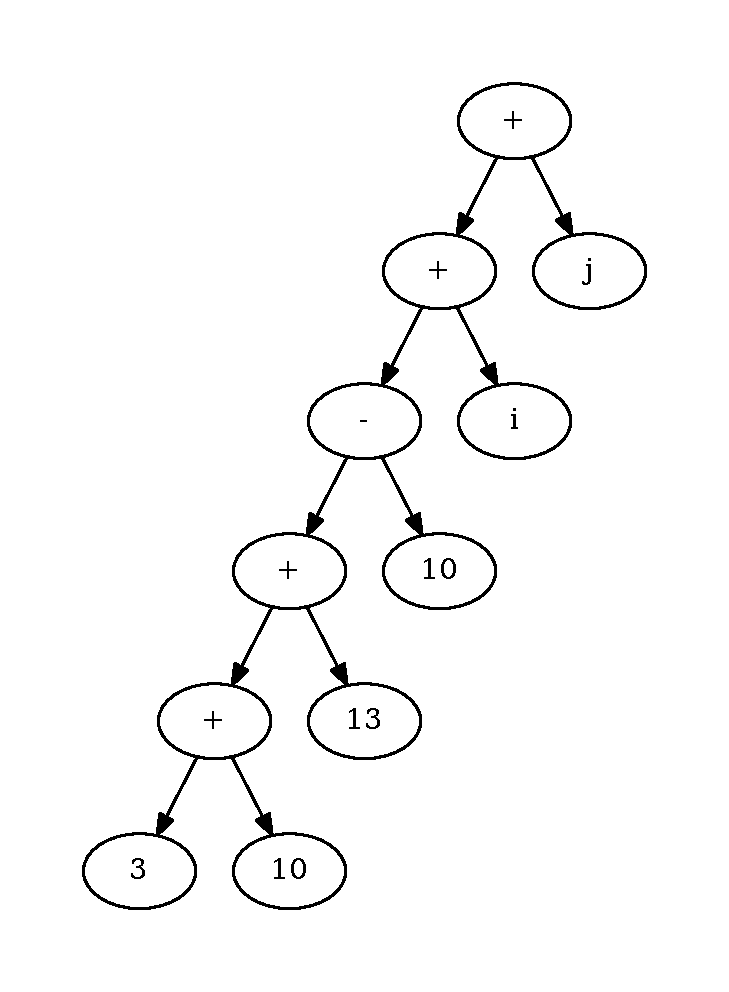
\includegraphics[scale=0.5]{graphs/optimalEvalTree.pdf}
\end{center}

The evaluator would then reduce this tree down to the following tree:

\begin{center}
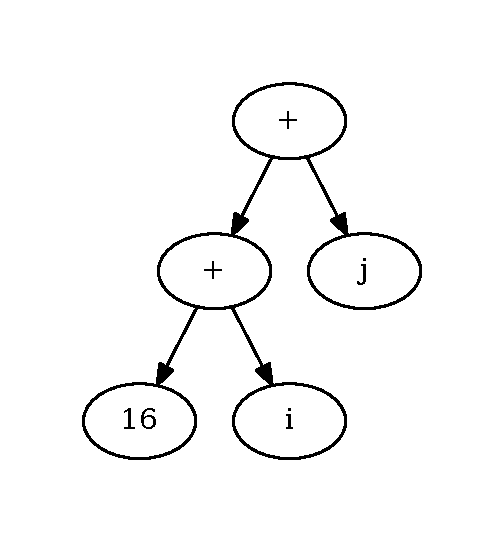
\includegraphics[scale=0.5]{graphs/optimalFullyEvalTree.pdf}
\end{center}

This generates much simpiler GPIR code:
\lstinputlisting[style=myGPIR]{code_samples/binaryOpImproved.td} 


\subsection{Pure Function Reduction}

When a function is pure (i.e. it contains no method calls
on kernel objects, and all arguments given to it when it is called can be evaluated at 
compile time) the function call should be able to be evaluated down to a single constant value.

The following GPC code is used as an example:

\lstinputlisting[style=myGPC]{code_samples/pureFun.gpc}

The function "f" does not call any methods on kernel objects, and has no arguments.
Every time "f" is called it returns the integer value "2". Therefore wherever f is called can
be replaced with the integer value "2". However the compiler generates the following GPIR code
for this example:

\lstinputlisting[style=myGPIR]{code_samples/pureFun.td}

When "f" is called its value is stored in a register. This is currently how function calls
store their return value when evaluated. An improvement to function evaluation to support
reduction of "pure functions" would result in generating this simpler GPIR code:

\lstinputlisting[style=myGPIR]{code_samples/pureFunImproved.td}


\subsection{Register Tracking}
As explained in section {insert section}, the register tracking is non existent and every
time a new value needs to be stored the register counter is just updated. After a while this
could possibly use a lot of memory. A more efficient method would be to track registers
being used, once a variable goes out of scope then that register gets "freed".

The "free list" can be implemented in Haskell as a simple linked list containing the numbers
of registers that are free. Every time a register is "freed" its number gets added
to the tail of the queue. When attempting to assign a variable a register the list is checked
to see if it has any free registers on it, if it is then the head of the queue is taken
as the register number. Otherwise the total register counter is incremented and the new value
is used as the register number.

In a scope keep track of all the register numbers allocated, once out of scope then add every
one of those numbers to the "free list", as the values in those register will not need
to be used again. This method of register tracking and freeing will use far less total
registers than using a new register for each value.

